\documentclass[journal]{IEEEtran}
\usepackage{amsthm}
\newtheorem{definition}{Definition}

\usepackage{booktabs}
\usepackage[table]{xcolor}
\usepackage{pgfplots}
\pgfplotsset{compat=1.18}
%\usepackage{subcaption}
\usepackage{graphicx}
\usepackage{xcolor}
\usepackage{colortbl}
\usepackage{contour}
\contourlength{0.8pt} % thickness of the halo

\usepackage{amssymb}
%\usepackage{hyperref}
\usepackage[utf8]{inputenc}
%\usepackage[hidelinks]{hyperref}
\usepackage{url}
\usepackage{cite}
\usepackage{enumitem}
%\usepackage{subfig}
\usepackage{subfigure}
\usepackage{amsmath}
\usepackage{algorithm}
\usepackage{algpseudocode}
%\usepackage{caption}
\usepackage{pgf-pie}
\usepackage{pgfplots}
\usepgfplotslibrary{dateplot}
\usepgfplotslibrary{units}
\pgfplotsset{compat=1.18}
\usepackage{tabularx}
\usepackage{booktabs}
\usepackage{minted}
\usemintedstyle{borland}
\usepackage{comment}
\usepackage{pgf-pie}
\usepackage[obeyclassoptions,mode=buildnew]{standalone}

\usetikzlibrary{arrows.meta, positioning, calc}

% darken the colors a little bit
\definecolor{red}  {rgb}{0.9,0.0,0.0}
\definecolor{green}{rgb}{0.0,0.7,0.0}
\definecolor{blue} {rgb}{0.0,0.0,0.9}

\definecolor{OkabeBlue}{RGB}{0,114,178}
\definecolor{OkabeOrange}{RGB}{213,94,0}
\definecolor{OkabeGreen}{RGB}{0,158,115}
\definecolor{OkabeSky}{RGB}{86,180,233}
\definecolor{OkabeVermilion}{RGB}{230,159,0}

\definecolor{OIblue}{HTML}{0072B2}
\definecolor{OIorange}{HTML}{E69F00}
\definecolor{OIgrey}{HTML}{999999}

\newcommand{\arad}[1]{\textcolor{orange}{Arad: #1}}
\newcommand{\ori}[1]{\textcolor{blue}{Ori: #1}}
\newcommand{\discuss}[1]{\textcolor{blue}{#1}}
\newcommand{\red}[1]{\textcolor{red}{#1}}
\newcommand{\blue}[1]{\textcolor{green}{#1}}
\newcommand{\extended}[1]{}

\usepackage[most]{tcolorbox}

% \usepackage{authblk}

\title{Profitable Liquidity Provision: Mitigating DeFi Impermanent Loss through Correlation and Turnover Analysis}
\author{}
%\institute{}

% \author{
% \IEEEauthorblockN{Arad Kotzer, Ori Rottenstreich}
% \IEEEauthorblockA{%\textit{Department of Computer Science } \\
% Technion - Israel Institute of Technology\\
% %Haifa, Israel \\
% emails: aradk@cs.technion.ac.il, or@technion.ac.il
% }
% }

\begin{document}

\maketitle

\begin{abstract}
Liquidity provision in automated market makers (AMMs) is often described as passive yield farming, yet liquidity providers (LPs) frequently underperform a simple buy-and-hold (HODL) benchmark due to impermanent loss (IL). 
This paper develops a practical, data-driven framework for evaluating and mitigating IL risk in Uniswap v3 pools using distributional and predictability metrics derived from historical price divergence. Using pool-level observations from eight major Uniswap v3 pools over roughly 4.5 years, we construct monthly price-ratio samples aligned with realistic holding horizons and summarize IL exposure via (i) a non-parametric downside bound based on the 5--95\% percentiles, (ii) median- and mean-implied IL and (iii) a standard-deviation-based boundary. To capture the temporal persistence of divergence, we model the log price ratio with an AR(1) specification and report the implied half-life as a horizon proxy for how long IL episodes tend to persist.
Empirically, we find that pools separate into distinct IL risk tiers driven primarily by \emph{asset correlation} rather than absolute volatility. Correlated volatile--volatile pairs exhibit near-zero typical monthly IL and comparatively mild downside bounds, while stable--volatile pairs display the most systematic IL drag. A recursive backtest indicates heterogeneous calibration across pools, consistent with fat-tailed divergence risk. 
Finally, we translate these findings into operational guidance for pool selection and horizon management, illustrating how risk-aware selection based on IL metrics and turnover can improve expected net performance relative to naive fee-tier heuristics. \ori{abstract is quite long and technical, you can omit 1-2 sentences or details if needed}
\end{abstract} 


%\keywords{Blockchain, DeFi, Impermanent Loss, Automated Market Makers}

\pagestyle{plain}
\thispagestyle{empty}

\section{Introduction}

The Decentralized Finance (DeFi) ecosystem comprises various financial services that run as blockchain applications~\cite{schar2021decentralized, zetzsche2020decentralized, jensen2021introduction, Bitcoin, wood2014ethereum}. DeFi enables participants to earn yield by providing services (e.g., lending assets for interest or supplying liquidity for fees). The core strategies revolve around lending money for interest and providing liquidity to token exchanges for transaction fees. They also include generating actions on DeFi platforms to earn engagement rewards. Current \ori{ maybe say 'Recent'?} estimates of the DeFi token market cap range from approximately 90 billion USD~\cite{forbes2025defi} to 103 billion~\cite{coingecko2025defi}, as of December 2025.

However, the prevailing narrative that liquidity provision is a passive "yield farming" strategy is increasingly challenged by the reality of \textit{Impermanent Loss} (IL). IL represents the shortfall between the value of an LP’s pool position and the value of simply holding the same tokens (HODL). When the relative prices of pooled assets diverge, \ori{I think the next part is confusing and suggest rephrasing} the AMM algorithm sells the outperforming asset to buy the underperforming one, reducing the LP's total position value relative to the market.

Crucially, empirical evidence suggests that for many LPs, the fee income generated is insufficient to compensate for this structural drag. In a landmark study of 17 popular Uniswap v2 pools, Loesch et al.~\cite{loesch2021impermanent} demonstrated that total fees earned (199M USD) failed to offset IL, resulting in an aggregate underperformance of 61M USD compared to the HODL strategy (\ori{add 'potential revenue of'? as it indicates the change in HODL and not HODL value} 261M USD). This implies a yield trap: LPs often chase high nominal APYs in volatile pools, unaware that the \textit{Net Profit}—defined as \ori{fees? (without capital)} Fees minus IL—is negative.

In this paper, \textit{we present a statistical framework for maximizing LP profitability by quantifying and mitigating IL risk}. We analyze historical data from eight major Uniswap v3 pools \ori{add 'for'?} over 4.5 years (May 2021--December 2025) to characterize the stochastic behavior of price divergence. Unlike previous studies that focus primarily on theoretical derivation, we introduce actionable, data-driven metrics designed to aid decision-making under uncertainty. Specifically, we utilize the \textit{5–95\% Downside Bound} ($IL_{bound}$) to capture tail risk in leptokurtic \ori{maybe be easier with the readers :)} (fat-tailed) crypto markets, and the \textit{Half-Life} ($HL$) of mean reversion to quantify the minimum necessary liquidity lock-up period.

\ori{maybe say you categorize cryptocurrencies or this is clear from the next sentence?}
Our analysis reveals that pools fall into distinct risk tiers driven by asset correlation rather than absolute volatility. We demonstrate that volatile-volatile pairs (e.g., WBTC/WETH) often exhibit lower IL risk than stable-volatile pairs (e.g., WETH/USDT) due to high correlation buffers \ori{what are buffers here?}. Based on these findings, we derive a set of operational rules for pool selection, showing that maximizing fee velocity and matching investment horizons to statistical half-lives are more predictive of net profit than the fee tier alone.
In out-of-sample testing spanning 2022--2025, our metric-guided pool selection yielded a total net gain of 77.38\%, outperforming simple pool averages by over 30\% and the HODL benchmark by more than 10-fold. These results provide LPs with the tools to navigate the trade-off between fee accumulation and capital preservation in an objective, risk-aware manner.

The remainder of this paper is organized as follows. Section~\ref{sec:background} provides the necessary background on AMMs and IL. \ori{you skip III here and dives into subsections of IV} Section~\ref{sec:general_statistics} introduces our statistical methodology, defining the mean-variance, non-parametric percentile, and mean-reversion metrics used to quantify risk. Section~\ref{sec:empirical_analysis} presents the empirical analysis of eight real-world Uniswap v3 pools, applying these metrics to historical data to uncover risk tiers and temporal dynamics. Section~\ref{sec:discussion} discusses the practical implications of these findings, proposing operational rules for pool selection and demonstrating their economic impact through a comparative case study. Finally, Section~\ref{sec:conclusion} concludes the paper and outlines directions for future research.


\section{Background}
\label{sec:background}
\subsection{AMM (Automated Market Maker)}
Automated Market Makers (AMMs)~\cite{hertzog2017bancor} are decentralized exchange protocols that enable coin exchange using liquidity pools. 
The most common AMMs type is \emph{constant function market makers} (CFMMs), where a trading function $f(x_0,x_1)$ imposes an invariant on token reserves $x_0, x_1$.
The most prominent example is the constant-product rule $x_0 \cdot x_1 = K$ used by Uniswap v2 \ori{add where $x_0, x_1$ indicate ...}. Generalizations include weighted geometric means (Balancer) and stableswap hybrids that blend constant product and sum (Curve)~\cite{bartoletti2022theory}.


AMMs effectively act as \emph{algorithmic price oracles}. Whenever the pool price deviates from external markets, arbitrage restores alignment~\cite{angeris2020improved}. 
Arbitrage thus plays the role of a stabilizing mechanism and a source of value extraction~\cite{pusceddu2024lean}.
This arbitrage-based alignment sustains on-chain liquidity and also determines value transfers. Traders may pay \emph{slippage} (execution worse than the pre-trade marginal price), \ori{is the following needed? you explain IL later} and LPs may incur \emph{impermanent loss} when the post-trade reserve mix underperforms HODL. Moreover, adversarial ordering (front-running, sandwiching~\cite{heimbach2022eliminating, zhou2021high}) can extract value under \emph{maximal extractable value} (MEV) \cite{mazorra2022price, daian2020flash, qin2021mev}.

% However, MEV from transaction ordering (front-running, sandwiching) is a separate phenomenon and not part of IL’s definition~\cite{qin2021mev}.


% AMMs effectively act as \emph{algorithmic price oracles}. whenever the pool price deviates from external markets, arbitrage restores alignment~\cite{angeris2020improved}. This mechanism explains both continuous liquidity and value transfer channels (e.g., slippage for traders, IL for LPs). Adversarial effects such as front-running and \emph{maximal extractable value} (MEV) arise from transaction ordering but are orthogonal to the definition of IL~\cite{qin2021mev}.

% A key insight is that AMMs act as \emph{algorithmic price oracles}. Rational traders exploit arbitrage opportunities when pool prices deviate from external market rates. This aligns the AMM’s internal exchange rate with global reference prices~\cite{angeris2020improved}. This arbitrage game underpins the economic mechanism of AMMs, ensuring that even without trusted intermediaries, prices converge towards consistency across markets. Formalizations of this property show that swaps yield positive gain precisely when the pool’s swap rate diverges from the oracle price. Arbitrage thus plays a role of stabilizing mechanism and a source of value extraction~\cite{pusceddu2024lean}.

% AMMs have also become a focal point for adversarial strategies. Transaction-ordering attacks, such as front-running and sandwich trades, exploit miners’ or validators’ control over transaction sequencing, extracting value at the expense of ordinary users~\cite{qin2021mev}. The widespread incidence of such \emph{maximal extractable value} (MEV) highlights the importance of rigorous economic modeling and verification of AMMs to ensure robustness in adversarial environments.

% Overall, AMMs represent both a practical and theoretical cornerstone of DeFi: they provide decentralized liquidity through simple, composable mechanisms, while raising deep questions about market efficiency, incentive compatibility, and security. Their study thus requires an interdisciplinary approach spanning economics, game theory, and formal methods.


\subsection{Liquidity Provision}
\label{sec:liquidity-provision}

Liquidity provision is the process by which users deposit tokens into an AMM pool, enabling traders to swap assets directly against pooled reserves. In return, \textit{liquidity providers} (LPs) receive a proportional share of the pool’s swap fees~\cite{gogol2024sok, chiu2023fragility, saengchote2023decentralized}.
For example, in a pool of Uniswap v2 ETH / USDC, LPs deposit equal values of ETH and USDC. Traders then exchange one asset for the other via the constant product invariant of the pool. This mechanism underpins decentralized exchanges by providing continuous on-chain liquidity without order books.
Figure~\ref{fig:pool_illustration} illustrates the liquidity provision flow. First, an LP deposits amounts $(x_0,x_1)$ of assets $(c_0,c_1)$ into the pool. When a trader swaps, the pool balances change along the pricing curve, updating the implied price. Finally, upon withdrawal, the LP receives her new proportional mix of tokens plus the fees accrued to the position.

\begin{figure}[h]
\centering
\resizebox{\linewidth}{!}{%
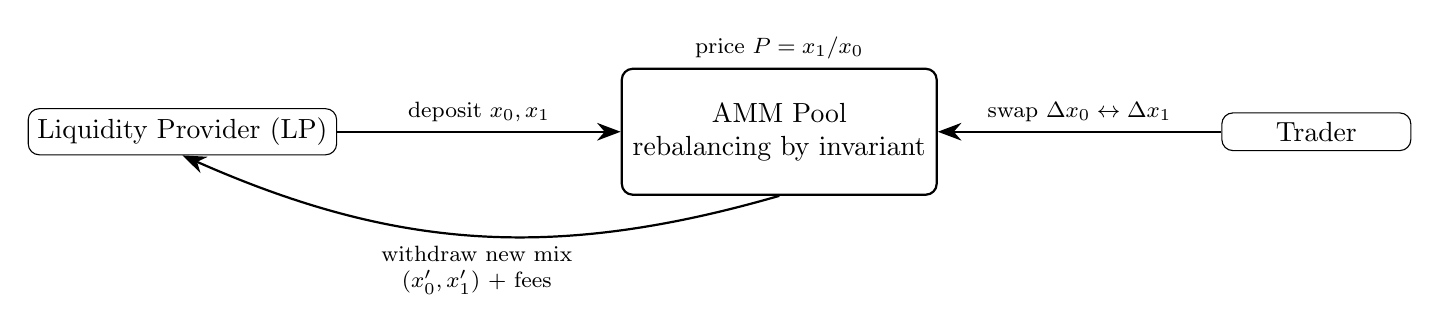
\begin{tikzpicture}[
  >={Stealth[length=3mm]},
  node distance=2.2cm,
  pool/.style={rectangle, rounded corners, draw, thick, minimum width=4cm, minimum height=1.6cm, align=center},
  role/.style={rectangle, draw, rounded corners, minimum width=2.4cm, align=center},
  lab/.style={font=\footnotesize}
]

% Nodes
\node[role] (lp) {Liquidity Provider (LP)};
\node[pool, right=3.6cm of lp] (amm) {AMM Pool\\rebalancing by invariant};
\node[role, right=3.6cm of amm] (trader) {Trader};

% LP deposit & LP tokens
\draw[->, thick] (lp.east) -- node[lab, above] {deposit $x_0, x_1$} (amm.west);
% \draw[<-, thick] ($(amm.west)+(0, -0.35)$) -- node[lab, below] {mint LP tokens} ($(lp.east)+(0, -0.35)$);

% Trader swap & fees
\draw[->, thick] (trader.west) -- node[lab, above] {swap $\Delta x_0 \leftrightarrow \Delta x_1$} (amm.east);
% \draw[->, thick, shorten >=2pt] ($(amm.east)+(0,-0.35)$) -- ++(0.9, -0.7)
%   node[lab, right, align=left] {fees accrue\\to pool};

% Withdraw
\draw[<-, thick, bend right=20] (lp.south) to node[lab, below, align=center] {withdraw new mix\\($x'_0, x'_1$) + fees} (amm.south);

% Annotations inside pool
\node[lab] at ($(amm.north)+(0,0.25)$) {price $P = x_1/x_0$};

\end{tikzpicture}%
}
\caption{Liquidity provision illustration of a constant-product AMM}
\label{fig:pool_illustration}
\end{figure}


\begin{figure}[h!]
\centering
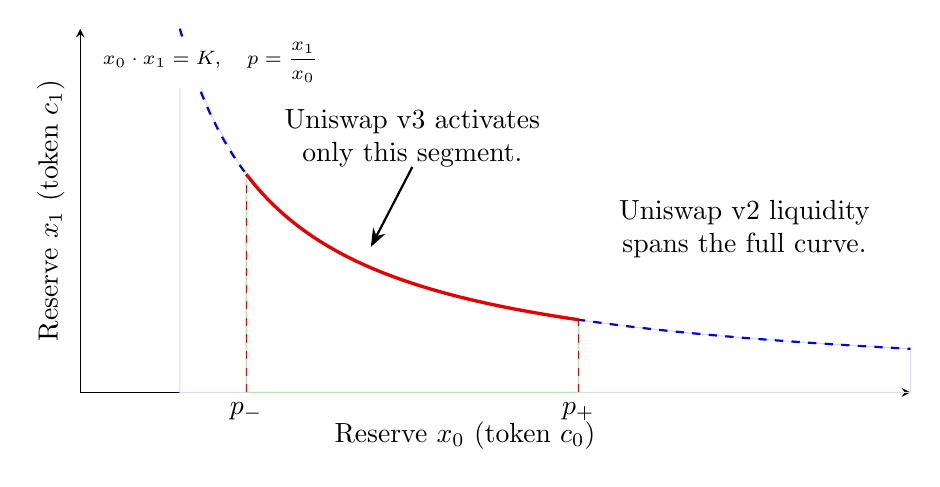
\begin{tikzpicture}[
  fill_v2/.style={blue!15, fill opacity=0.8},
  fill_v3/.style={green!30, fill opacity=0.8},
  plot_curve/.style={blue, thick},
  highlight_curve/.style={red, very thick},
]
\begin{axis}[
  xlabel={Reserve $x_0$ (token $c_0$)},
  ylabel={Reserve $x_1$ (token $c_1$)},
  axis lines=left,
  xmin=0, xmax=10,
  ymin=0, ymax=10,
  width=\linewidth, height=6.2cm,
  xtick=\empty, ytick=\empty,
  enlargelimits=false,
  clip=false,
  xlabel style={anchor=north, yshift=-5pt, xshift=-11pt},
  ylabel style={anchor=south},
]

% price band:
\def\pmin{2}
\def\pmax{6}

% v2 (full range)
\addplot [fill_v2, domain=1.2:10] {12/x} \closedcycle;

% v3 (concentrated range)
\addplot [fill_v3, domain=\pmin:\pmax] {12/x} \closedcycle;

% full bonding curve
\addplot [plot_curve, dashed, domain=1.2:10, samples=100] {12/x};

% active v3 segment
\addplot [highlight_curve, domain=\pmin:\pmax, samples=100] {12/x};

% price band markers
\draw[red, dashed] (axis cs:\pmin, 0) node[below=0.01pt, black] {\(p_{-}\)} -- (axis cs:\pmin, {12/\pmin});
\draw[red, dashed] (axis cs:\pmax, 0) node[below=0.01pt, black] {\(p_{+}\)} -- (axis cs:\pmax, {12/\pmax});

% labels (avoid “price” wording)
\node[text width=3.2cm, align=center] at (axis cs:8,4.5)
  {Uniswap v2 liquidity spans the full curve.};
\node[text width=3.5cm, align=center] at (axis cs:4,7)
  {Uniswap v3 activates only this segment.};
\draw[-Stealth, thick] (axis cs:4,6.2) -- (axis cs:3.5,4);

% small note: price definition
\node[anchor=north west, font=\scriptsize, fill=white, rounded corners=1pt, inner sep=2pt]
  at (rel axis cs:0.02,0.98) {$x_0 \cdot x_1=K,\quad p=\dfrac{x_1}{x_0}$};

\end{axis}
\end{tikzpicture}
\caption{Liquidity distribution in Uniswap v2 (full range) vs.\ Uniswap v3 (concentrated in \([p_{-},p_{+}]\)). The curve shows a constant-product contour \(x_0 \cdot x_1=K\), and the highlighted segment marks the price band where v3 liquidity is active.}
\label{fig:uniswap_fee_policy}
\end{figure}



\paragraph{Fee microstructure and concentrated liquidity.} \ori{avoid both . and : (see pdf). Also, your format for subsubsections here ussed a) and next subsection uses 1) and 2)}
AMM protocols differ in how fees interact with liquidity.
In Uniswap v2, swap fees are \emph{reinvested into the pool reserves} on each trade, so the product $x_0 \cdot x_1{=}K$ grows.
In Uniswap v3, fees are added to the \emph{separate fee counters} of each position and do not change the active liquidity $L$ \ori{how is $L$ related to $x_0$, $x_1$? explain} or the reserves until the LP explicitly claims or reinvests them. \ori{say in the text how price $p$ relates to $x_0$, $x_1$? you have it in Fig. 2}
Moreover, v3 allows LPs to choose a price band $[p_{-},p_{+}]$ and provide liquidity only inside it. When $p_{\text{pool}}\in[p_{-},p_{+}]$, the position behaves locally like a Constant Product Market Maker (CPMM) with "virtual" reserves determined by $[p_{-},p_{+}]$ and its liquidity $L$, and it earns fees. If price exits this band, the position converts to a single asset \ori{the position converts to a single asset - do you mean it allow exchanging in one direction only?} ($c_{0}$ if $p_{\text{pool}}<p_{-}$, $c_{1}$ if $p_{\text{pool}}>p_{+}$) and \emph{accrues no fees} until price re-enters or the LP rebalances. Figure~\ref{fig:uniswap_fee_policy} illustrates the liquidity distribution in Uniswap v2 and v3.




\subsection{Impermanent Loss}
\label{sec:background_il}

\emph{Impermanent Loss} (IL) is the fundamental risk exposure for liquidity providers in CFMMs. It is defined as the relative underperformance of an LP's pool position compared to a passive buy-and-hold (\emph{HODL}) strategy of the same initial assets~\cite{evans2021liquidity, aoyagi2020liquidity}.

\subsubsection{Mechanism and Formalization}
IL arises from the convex payout structure of the AMM invariant. When the relative market price of the pooled tokens changes, arbitrageurs trade against the pool to realign its internal price with external markets. This process forces the AMM to sell the appreciating asset and buy the depreciating asset, systematically reducing the total value of the pool relative to the HODL benchmark.
For a standard CPMM like Uniswap v2, where reserves $x_0, x_1$ satisfy $x_0 \cdot x_1 = K$, Tiruviluamala et al.~\cite{tiruviluamala2022general} \ori{derived} derive the canonical closed-form expression for IL as a function of the price ratio change $R = p'/p$:
\ori{this might be hard to change, but I think of a loss in positive values while consistently it is described as the value change which is negative. Any ideas to clarify that?}
\begin{equation}
    \mathrm{IL}(R) = \frac{2\sqrt{R}}{1+R} - 1.
    \label{eq:il_canonical}
\end{equation}

This function is always non-positive ($\mathrm{IL} \le 0$) and symmetric with respect to log-returns, implying that LPs incur losses regardless of the direction of price divergence. While the loss is referred to as impermanent because it theoretically vanishes if prices return to their initial ratio ($R=1$ \ori{maybe say instead: namely, $IL(R)=0$ for $R=1$?}), the path-dependent nature of volatility often crystallizes these losses upon withdrawal.

\subsubsection{Empirical Severity}
The theoretical guarantee that $IL \le 0$ has been validated by extensive empirical research, though the extent to which fees offset this loss varies by market regime. Early analysis of Uniswap v2 by Heimbach et al.~\cite{heimbach2021behavior} and Boueri et al.~\cite{boueri2021g3m} established that while stablecoin pools provide consistent returns, pools consisting of volatile or exotic pairs suffer from severe IL that frequently exceeds fee income. This structural underperformance is amplified in concentrated liquidity models. Heimbach et al.~\cite{heimbach2022risks} found that in Uniswap v3, narrow liquidity ranges increase exposure to divergence, resulting in net losses for a significant majority of passive positions in volatile pairs.
Conversely, recent work by Roman et al.~\cite{roman2025impact} introduces a more nuanced perspective, demonstrating that when trading fees are high relative to volatility, positions can experience \textit{Impermanent Gain} during small price fluctuations. However, they conclude that this protective effect is often insufficient during larger divergence events typical of crypto markets. Collectively, these studies~\cite{heimbach2021behavior, boueri2021g3m, heimbach2022risks, roman2025impact} confirm that for uncorrelated assets, IL remains a dominant risk factor that requires active statistical management.


\section{Statistic Models Metrics \ori{check if it is more common to use statistic or statistical? statistic mighe be fine}}
\label{sec:metrics}

defined IL deterministically \ori{in this you mean by looking backward based on real price changes unlike estimates for future changes? clarify}, LPs must assess the \textit{probability} and \textit{duration} of price divergence in stochastic markets. To quantify this, we analyze historical data using three complementary metrics:
\begin{enumerate}
    \item \textbf{Mean-Variance Analysis:} Uses standard deviation to define typical risk boundaries.
    \item \textbf{Tail Risk (5–95\%) Analysis:} Captures extreme events (leptokurtosis) common \ori{extreme and common are somehow confusing? maybe reasonable is better?} in crypto markets.
    \item \textbf{Mean Reversion Analysis:} Estimates the speed of price recovery to determine optimal lock-up periods.
\end{enumerate}

Since IL is realized over a holding horizon, we define the normalized price ratio over \ori{in $h$ periods, do you mean of length $h$?, later you use - and here not? are the time periods disjoint? do they start at $t$ for various $t$? clarify } \(h\) periods as:
$$
    R^{(h)}_{t} \;=\; \frac{p_{t+h}}{p_t}.
$$
The metrics below are computed from the empirical distribution \(\mathcal{H}_{R^{(h)}}\) induced by the historical series \(\{R^{(h)}_{t}\}\).


\subsection{Mean and Standard Deviation Analysis}
A traditional statistical approach to characterizing the distribution of the price ratio \(R^{(h)}\) involves its mean \(\mu_{R^{(h)}}\) and standard deviation \(\sigma_{R^{(h)}}\). These two moments are the cornerstone of classical statistical analysis and are fundamental to many models in finance, most notably in Modern Portfolio Theory, where they are used to define expected return and risk~\cite{markowitz1952portfolio, ross2014introduction}.

Following this paradigm, we define the expected IL based on the historical average of the \(h\)-period price ratio, \(\mu_{R^{(h)}}\): 
\begin{equation}
\label{eq:il_mean}
\mathrm{IL}_{\text{mean}} = \frac{2\sqrt{\mu_{R^{(h)}}}}{1+\mu_{R^{(h)}}} - 1.
\end{equation}
\ori{in the above, one could also have in mind, mean value of the IL (for various $R$ values) rather than IL (mean R). Can you justify?}

To establish a risk boundary, a one-standard-deviation interval \([\mu_{R^{(h)}}-\sigma_{R^{(h)}},\, \mu_{R^{(h)}}+\sigma_{R^{(h)}}]\) is commonly used to represent the range of expected variation. We define a standard-deviation-based IL boundary, \(\mathrm{IL}_{\sigma\text{-bound}}\), by evaluating IL at the edges of this range \ori{explain why $min$? you take the more largest in absolute value?}:

\begin{equation}
\label{eq:il_sigma_bound}
\begin{aligned}
\mathrm{IL}_{\sigma\text{-bound}}
= \min\Biggl(
&\frac{2\sqrt{\mu_{R^{(h)}} - \sigma_{R^{(h)}}}}{1+\bigl(\mu_{R^{(h)}} - \sigma_{R^{(h)}}\bigr)} - 1, \\
&\frac{2\sqrt{\mu_{R^{(h)}} + \sigma_{R^{(h)}}}}{1+\bigl(\mu_{R^{(h)}} + \sigma_{R^{(h)}}\bigr)} - 1
\Biggr).
\end{aligned}
\end{equation}


We note this approach relies on the implicit assumption that \(\mathcal{H}_{R^{(h)}}\) is reasonably symmetric and well-behaved. 
It is well-documented that financial return distributions can exhibit significant skewness and heavy tails (leptokurtosis), properties that are not adequately captured by the mean and standard deviation alone~\cite{mandelbrot2004fractals}. In such cases, the standard deviation may underestimate the probability of extreme events, motivating the use of non-parametric methods that are more robust to such distributional properties.
\textit{To conclude, this metric captures the pool’s \emph{typical} IL environment.}

\subsection{The 5--95 Percentile Metric}

To address the limitations of a mean-variance approach, particularly its sensitivity to outliers and its implicit assumptions regarding the data's distribution, we employ the non-parametric 5--95 percentile metric. 
We apply this metric to the empirical distribution of the \(h\)-period price ratio \(R^{(h)}\). Let \(\mathcal{H}_{R^{(h)}}\) be the distribution derived from historical data over the chosen estimation window. We identify the 5th and 95th percentiles of this distribution, denoted \(R^{(h)}_{0.05}\) and \(R^{(h)}_{0.95}\), respectively. The corresponding IL boundary, \(\mathrm{IL}_{\text{bound}}\), is defined by the most severe loss at these percentile extremes:
\ori{actually, are these values (including the previous one) a function of $t$?}
\begin{equation}
\label{eq:il_bound}
\mathrm{IL}_{\text{bound}} = \min\left(
\frac{2\sqrt{R^{(h)}_{0.05}}}{1+R^{(h)}_{0.05}} - 1,\quad
\frac{2\sqrt{R^{(h)}_{0.95}}}{1+R^{(h)}_{0.95}} - 1
\right).
\end{equation}
This approach yields a quantifiable downside threshold representing the maximum impermanent loss an LP should expect to face in 90\% of observed \(h\)-period scenarios.

Furthermore, we approximate the typical IL by using the median of \(\mathcal{H}_{R^{(h)}}\), denoted \(R^{(h)}_{\text{median}}\). The median-approximated IL is:
\begin{equation}
\label{eq:il_median}
\mathrm{IL}_{\text{median}} = \frac{2\sqrt{R^{(h)}_{\text{median}}}}{1+R^{(h)}_{\text{median}}} - 1.
\end{equation}

\textit{To conclude, this metric captures downside IL risk under skewness and heavy tails by using empirical percentiles of \(R^{(h)}\) to produce a robust tail-loss boundary.}

\subsection{Mean-Reversion-Based Predictability Metric}
\label{subsubsec:mean_reversion_metric}

While the distributional metrics above summarize the \emph{magnitude} of IL risk, they do not describe how the price ratio evolves over time. 
For an LP, this temporal behavior matters: If relative prices revert quickly after shocks, IL episodes are more likely to be short-lived rather than persistent.
To quantify this \emph{predictability}, we study how fast the price ratio returns toward a typical level after a deviation. 
Let \(R_t\) denote the oriented price ratio sampled at the chosen frequency, and define the log-ratio \(    X_t = \log R_t \) \ori{is $X$ related to $x$ in the CPMM formula?}. 

\ori{the following was hard for me to follow. I suggest to explain in more words, e.g., like $\varepsilon$ and overall picture} We model \(X_t\) using a simple mean-reverting specification in which next period’s deviation from a long-run level \(\mu\) is proportional to today’s deviation:
$$
\label{eq:ar1_ratio}
X_{t+1} - \mu = \phi \bigl(X_t - \mu\bigr) + \varepsilon_{t+1}, 
\qquad \varepsilon_{t+1} \sim \text{i.i.d. } N(0, \sigma^2_\varepsilon).
$$
This is a first-order autoregressive model (AR(1)). The parameter \(\phi\) \ori{is $\phi$ a scalar? in the formula it seems like a function} measures \emph{persistence}: When \(|\phi|\) is close to 1, shocks decay slowly and deviations can last for many periods. When \(|\phi|\) is smaller, shocks fade quickly and the process reverts to \(\mu\) faster.

A convenient way to express the speed of reversion is the \emph{half-life} ($HL$), defined as the expected number of sampling periods required for a shock to \(X_t\) to shrink by 50\%:
\begin{equation}
\label{eq:half_life}
\text{HL} = -\frac{\ln 2}{\ln \phi}.
\end{equation}
$HL$ is reported in the units of the sampling frequency (e.g., days or months). 
We interpret pools with shorter half-lives as more predictable from an IL perspective, since relative-price deviations—and hence IL episodes—tend to dissipate within a foreseeable horizon.
\textit{To conclude, this metric captures how persistent relative-price shocks are, meaning how long IL episodes tend to last.}

\ori{Give some concluding sentence with a hint what to do with these metrics?}

\section{Empirical Analysis on Real Pools}
\label{sec:empirical_analysis}

\subsection{Data}


\begin{table}[t]
\centering
\scriptsize
\resizebox{0.5\textwidth}{!}{%
\begin{tabular}{lll}
\hline
Pool address & Tokens & Fee tier\\
\hline
\texttt{0x4e68ccd3e89f51c3074ca5072bbac773960dfa36} & WETH/USDT & 0.30\% \\
\texttt{0x11b815efb8f581194ae79006d24e0d814b7697f6} & WETH/USDT & 0.05\% \\
\texttt{0x9db9e0e53058c89e5b94e29621a205198648425b} & WBTC/USDT & 0.30\% \\
\texttt{0x4585fe77225b41b697c938b018e2ac67ac5a20c0} & WBTC/WETH & 0.05\% \\
\texttt{0xcbcdf9626bc03e24f779434178a73a0b4bad62ed} & WBTC/WETH & 0.30\% \\
\texttt{0x5ab53ee1d50eef2c1dd3d5402789cd27bb52c1bb} & AAVE/WETH & 0.30\% \\
\texttt{0xa6cc3c2531fdaa6ae1a3ca84c2855806728693e8} & LINK/WETH & 0.30\% \\
\texttt{0x1d42064fc4beb5f8aaf85f4617ae8b3b5b8bd801} & UNI/WETH & 0.30\% \\
\hline
\end{tabular}
}
\caption{Summary of Uniswap v3 pools used in the empirical analysis.}
\label{tab:pools}
\end{table}


We collect historical observations for eight major Uniswap v3 liquidity pools using The Graph's public \ori{what is Subgraph here? why in capital? is that the formal name?} Subgraph~\footnote{https://thegraph.com/explorer}, following the data construction procedure in \cite{loesch2021impermanent}. 
The sample spans roughly 4.5 years (May 2021--December 2025) and includes pools pairing WETH and WBTC against the dominant USD stablecoins (USDC/USDT), as well as WBTC/WETH pools, \ori{break into a new sentence, too long} across the 0.05\% and 0.30\% fee tiers. 
The paper \ori{which paper? [8] or our paper?} tracks the pool-implied price over time and forms the normalized price ratio series used to compute the IL. 
Table~\ref{tab:pools} summarizes the pool addresses, token pairs and fee tiers. \ori{do you want to list the tokens here as some like Link are not common}


\begin{figure}[ht]
    \centering
    \input{monthly_pools_tikz_transformed.tex}
    \caption{Monthly transformed closing price ratio $p$ for eight Uniswap V3 pools 5 years.}
    \label{fig:monthly_pools_transformed}
\end{figure}


\begin{figure}[t]
\centering
\resizebox{0.5\textwidth}{!}{%
    \input{monthly_pools_tvl}
}
\caption{Monthly total value locked (TVL, in USD).}
\label{fig:monthly_tvl}
\end{figure}




\begin{figure}[ht]
    \centering
    \resizebox{0.5\textwidth}{!}{%
        \input{monthly_pools_volume_tikz.tex}
    }
    \caption{Monthly total trading volume (in USD).}
    \label{fig:monthly_pools_volume}
\end{figure}




\subsection{General Pool Statistics}
\label{sec:general_statistics}
Figure~\ref{fig:monthly_pools_transformed} presents the monthly closing price series $p$ for each analyzed Uniswap v3 pool. First, we note the duplicated pairs (WETH--USDT and WBTC--USDT \ori{i was confused, is there more than one WBTC--USDT? }) exhibit nearly identical prices across their respective pools, even though each pool’s price is determined endogenously by its reserve ratio (and not directly by the market price). This is because arbitrage traders \ori{not sure 'who' is needed in this sentence} who trade against any deviation from the prevailing market price. Next, we observe the WETH--USDT pools (4e and 11) display a pronounced trough in mid-2022 (around June 2022), consistent with the sharp market drawdown in that period. By contrast, the WBTC--USDT pool (9d) evolves on a substantially larger scale and exhibits a different timing of its major decline (late 2022). Meanwhile, the cross-asset ratio pools (WBTC--WETH, AAVE--WETH, LINK--WETH, and UNI--WETH) remain on lower yet distinct levels with heterogeneous dynamics. Overall, the figure highlights the large dispersion in price scales and long-run trajectories across pools, which directly translates into different IL exposures.

Figure~\ref{fig:monthly_tvl} presents the monthly total value locked (TVL) of the pools. The highest liquidity is concentrated in the WBTC/WETH 0.30\% pool (cb) and the WETH/USDT 0.30\% pool (4e), which persistently remain in the $10^{8}$ USD regime: Pool cb reaches a peak of roughly $5\times10^{8}$ USD and then retraces, while pool 4e trends upward and peaks around $3.6\times10^{8}$ USD near the end of the sample. The corresponding lower-fee counterparts (45 for WBTC/WETH at 0.05\% and 11 for WETH/USDT at 0.05\%) start from substantially smaller bases and grow over time, with 11 and the WBTC/USDT pool (9d) both expanding to the $\sim10^{8}$ USD range in late 2024. Among the DeFi governance-token pools, LINK/WETH (a6) and UNI/WETH (1d) exhibit mid-range liquidity (typically $10^{7}$--$10^{8}$ USD), whereas AAVE/WETH (5a) remains comparatively smaller, topping out around a few $\times10^{7}$ USD. 

Figure~\ref{fig:monthly_pools_volume} presents the total monthly trading volume, measured in USD. The WETH/USDT pools (4e and 11) and the WBTC/WETH pools (45 and cb) dominate overall volume, with the low-fee WETH/USDT pool (11) exhibiting the highest typical activity (frequently in the $10^{9}$--$10^{10}$ USD range and peaking above $5\times10^{9}$ USD), while the DeFi governance-token pools (AAVE/WETH, LINK/WETH, UNI/WETH) and WBTC/USDT (9d) operate at materially lower levels on average. 

Comparing pools with the \emph{same token pair} but different fee tiers reveals a distinct trade-off between fee margin and capital velocity. While \emph{lower-fee} pools display systematically higher \emph{turnover} (monthly volume relative to TVL) due to order flow routing, this increased activity does not automatically result in higher returns. Specifically, to outperform a 0.30\% fee tier, a 0.05\% pool requires a turnover rate more than $6\times$ higher ($0.30/0.05$) than its high-fee counterpart.
Our data highlights divergent outcomes in this regard. For example, in May 2021, the WBTC/WETH 0.05\% pool (45) achieved a turnover of $\approx57\times$ compared to just $\approx5.4\times$ for the 0.30\% pool (cb). Since this ratio ($\approx 10.5\times$) exceeds the breakeven threshold of 6, the lower-fee pool was the superior choice. Conversely, for WETH/USDT in the same month, the 0.05\% pool (11) reached a turnover of $\approx77\times$ versus $\approx14\times$ for the 0.30\% pool (4e). Here, the turnover ratio ($\approx 5.5\times$) fell short of the threshold, meaning the 0.30\% pool generated a higher fee yield despite processing significantly less volume relative to its liquidity. This underscores that comparisons must account for the \emph{fee velocity} ($\text{Fee Rate} \times \text{Turnover}$) rather than relying on volume or fee tiers in isolation.



\subsection{IL and Money Loss In \ori{in} Practice}

\begin{figure}[ht]
  \centering
    \resizebox{0.5\textwidth}{!}{%
        \input{monthly_il}
    }
  \caption{Monthly pool IL.}
  \label{fig:monthly_il}
\end{figure}

\ori{you mix Fig. and Figure along the paper}
Figure~\ref{fig:monthly_il} reports the monthly IL. The two WETH/USDT pools (4e and 11) move almost identically and exhibit the largest systematic losses during the mid--2022 drawdown, reaching their worst month in June~2022 at $\approx$ $-3.91\%$ (4e) and $-3.90\%$ (11). In contrast, the correlated WBTC/WETH pools (45 and cb) experience only mild losses during June~2022 ($\approx$ $-0.16\%$) but display a clear regime shift in mid--2025: Both pools attain their maximum monthly loss in July~2025 at roughly $-1.33\%$, consistent with an idiosyncratic divergence between BTC and ETH rather than a broad market shock. The remaining pools populate an intermediate risk band, with WBTC/USDT (9d) and UNI/WETH (1d) showing comparatively larger drawdowns in June~2022 ($\approx$ $-2.56\%$ and $-2.58\%$, respectively), while LINK/WETH (a6) reaches its worst month later in May~2025 at $\approx-1.69\%$ and AAVE/WETH (5a) peaks in December~2024 at $\approx-3.24\%$. Overall, the figure reinforces that correlated pairs buffer against systemic crashes, yet all pools remain vulnerable to pair-specific dislocations that can generate sharp, localized IL.


IL is not limited to a theoretical loss of money, and in practice, when fee income is lower than IL, LP may exhibit net negative returns. In fact, \emph{all eight pools} exhibit such net-loss months, indicating that negative net returns are not isolated anomalies. For example, the WETH/USDT 0.30\% pool (4e) records a net loss of $\approx1.32\%$ in February~2024, where a fee yield of $\approx0.56\%$ is insufficient to offset $\approx1.88\%$ IL, while the WBTC/USDT pool (9d) experiences a net loss of $\approx0.62\%$ in January~2023 (fee yield $\approx0.65\%$ versus IL $\approx1.26\%$). Even correlated pairs are not immune: The WBTC/WETH 0.30\% pool (cb) suffers a net loss of $\approx1.25\%$ in July~2025 (fee yield $\approx0.08\%$ versus IL $\approx1.34\%$), consistent with a large pair-specific divergence.
These empirical observations highlight that \textit{IL  constitutes a structural and common operational risk, systematically challenging the assumption that passive fee generation guarantees positive net returns}.

\begin{table}[t]
\centering
\footnotesize
\begin{tabular}{lccccc}
\toprule
Pool & Fee tier & Month & Fee yield & IL & Net \\
\midrule
45 & 0.05\% & Jul 25 & 0.13\% & -1.33\% & -1.21\% \\
cb & 0.30\% & Jul 25 & 0.08\% & -1.34\% & -1.25\% \\
4e & 0.30\% & Feb 24 & 0.56\% & -1.88\% & -1.32\% \\
11 & 0.05\% & Jul 25 & 0.98\% & -2.19\% & -1.20\% \\
9d & 0.30\% & Jan 23 & 0.65\% & -1.26\% & -0.62\% \\
5a & 0.30\% & Jul 25 & 1.28\% & -2.24\% & -0.97\% \\
a6 & 0.30\% & May 25 & 0.50\% & -1.69\% & -1.18\% \\
1d & 0.30\% & June 22 & 1.28\% & -2.58\% & -1.30\% \\
\bottomrule
\end{tabular}
\caption{Pool net-loss examples.}
\label{tab:worst_net_loss}
\end{table}


\subsection{IL Metric Measurement}

\begin{figure}[ht]
    \centering
    \resizebox{0.5\textwidth}{!}{%
        \input{mean_std_R}
    }
    \caption{Mean and standard deviation of the monthly price ratio \(R^{(1m)}_t=p_{\mathrm{end}}/p_{\mathrm{start}}\).}
    \label{fig:mean_std_R}
\end{figure}



Fig.~\ref{fig:mean_std_R} presents the empirical mean and standard deviation of the monthly price ratio
\(R^{(1m)}_t = p_{\mathrm{end}}/p_{\mathrm{start}}\) of the pool.
Unlike Fig.~\ref{fig:monthly_pools_transformed}, this construction aligns with a one-month LP holding horizon by measuring within-month relative price movements.
Across pools, the mean ratios remain close to unity (approximately \(0.987\)–\(1.039\)), implying that typical monthly drift in the relative price is small compared to its dispersion.
The dispersion, however, varies substantially: The WETH/USDT pools (4e, 11) exhibit the largest month-to-month variability
(\(\sigma \approx 0.218\)–\(0.219\)), whereas the correlated WBTC/WETH pools (45, cb) are much more stable
(\(\sigma \approx 0.120\)).
The remaining pools fall in an intermediate band, with WBTC/USDT (9d) around \(\sigma \approx 0.161\) and the DeFi token pairs AAVE/WETH, LINK/WETH, and UNI/WETH (5a, a6, 1d) around \(\sigma \approx 0.168\)–\(0.173\).
Overall, this mean--variance view provides a horizon-consistent explanation for cross-pool IL differences: Pools with larger monthly dispersion in \(R^{(1m)}\) are more prone to severe IL realizations even when average drift is negligible.



\begin{figure}[t]
\centering
\resizebox{0.5\textwidth}{!}{%
        \input{pool_metric_analysis}
    }
\caption{Summary statistics computed over the monthly IL samples for each pool.}
\label{fig:monthly_il_summary_metrics}
\end{figure}


Fig.~\ref{fig:monthly_il_summary_metrics} summarizes the four monthly-IL risk metrics introduced in Section~\ref{sec:metrics}: $\mathrm{IL}_{\text{median}}$, $\mathrm{IL}_{\text{bound}}~(5\text{--}95)$, $\mathrm{IL}_{\sigma\text{-bound}}$, and $\mathrm{IL}_{\text{mean}}$. Two main trends emerge from this analysis. 
First, the metrics consistently separate the pools into clear risk tiers. The WBTC/WETH pools 45 and cb exhibit the smallest losses across all summaries. Their typical monthly IL is close to zero (medians $\approx-0.062\%$ and $\approx-0.054\%$) and their tail exposure is markedly milder than the rest (5--95 bounds around $-0.70\%$). At the opposite end, the WETH/USDT pools 4e and 11 display the largest systematic IL, with the most negative means (both $\approx$ $-0.367\%$) and the deepest downside bounds (5--95 bounds near $-1.87\%$ and $\sigma$-bounds around $-1.17\%$). The remaining pools form an intermediate regime: 9d, 5a, a6, and 1d have medians between roughly $-0.13\%$ and $-0.22\%$, while their downside bounds are substantially less severe than the WETH/USDT group (5--95 bounds between $\approx$ $-1.19\%$ and $-1.42\%$), indicating meaningfully smaller tail risk despite non-negligible typical IL.

The second trend is that the four metrics emphasize different aspects of IL risk and can therefore alter the relative ranking within the intermediate tier. 
For example, 1d has the most negative median among the intermediate pools ($\approx$ $-0.217\%$), suggesting worse ``typical'' months, yet its downside bound is the shallowest in that tier (5--95 bound $\approx-1.19\%$), implying comparatively stronger tail protection. Conversely, 9d has a less negative median ($\approx$ $-0.133\%$) but a deeper 5--95 bound ($\approx$ $-1.42\%$), reflecting more pronounced adverse-month exposure. 
Similarly, a6 and 5a have comparable means ($\approx$ $-0.243\%$ and $-0.240\%$) but differ in tail behavior (5--95 bounds $\approx-1.27\%$ versus $\approx-1.35\%$), illustrating that pools can share similar average IL while differing in the severity of rare dislocations. 
Overall, these cross-metric differences highlight that the preferred summary should match the LP’s objective---typical performance (median) versus downside protection (bounds) and shock sensitivity (mean).




\begin{figure}[ht]
\centering
\resizebox{0.5\textwidth}{!}{%
        \input{half_life_180_days}
    }
\caption{Mean 180-day rolling half-life of each pool, with the corresponding mean AR(1) coefficient $\phi$.}
\label{fig:half_life_180d_mean_phi_inside}
\end{figure}

Figure~\ref{fig:half_life_180d_mean_phi_inside} illustrates the medium-term predictability of each liquidity pool by plotting the mean 180-day rolling half-life of adjusted log prices. In this visualization, the bar length serves as a proxy for persistence---quantifying the average time required for a price shock to dissipate by half---while the corresponding mean AR(1) coefficient, $\phi$, is noted within each bar. These metrics are derived from overlapping 180-day windows. For each pool, we construct an adjusted price series $P_{\text{adj},t}$ (inverted where the mean is below unity) and fit an AR(1) model to the log prices, $X_t=\ln P_{\text{adj},t}$. The resulting window-specific coefficients $\phi_t$ are converted into half-lives ($HL$) via $\mathrm{HL}_t=-\ln 2 / \ln \phi_t$. The bar length represents the average $\mathrm{HL}_t$ across all valid windows, while the displayed $\phi$ is the simple mean of the AR(1) coefficients.

The results indicate that price deviations in these markets are persistent, but the extent of persistence differs materially across pools. Mean $HL$ range from about $43.33$ to $64.26$ days, while mean AR(1) coefficients span approximately $0.930$ to $0.974$, implying that shocks to the price ratio typically decay over several weeks to roughly two months. A key feature is that the mapping from $\phi$ to half-life is highly nonlinear as $\phi \to 1$, so even small differences in average persistence can translate into meaningful differences in expected shock duration. In the present sample this is most clearly reflected by the top-ranked pool 0x9d (WBTC/USDT), which attains the longest mean half-life ($64.26$ days) despite having a mean coefficient ($\phi\approx0.973$) comparable to several other pools (e.g., 0x4e and 0x11), highlighting that prolonged near-unit-root episodes in some windows can disproportionately inflate average half-life even when mean $\phi$ values appear similar.

Disaggregating by pool type reveals an updated cross-sectional pattern. The WBTC/USDT pool 0x9d is the most persistent market by a wide margin, suggesting that deviations between Bitcoin and the dollar-pegged asset can remain ``sticky'' for extended periods, potentially sustaining IL exposure over longer horizons. In contrast, the two WBTC/WETH pools (0x45, 0xcb) sit at the bottom of the ranking (mean $HL$ $\approx 43$--$44$ days), consistent with faster relative adjustment between two major crypto-assets. The WETH/USDT pools (0x11, 0x4e) form an intermediate cluster around $\approx 47$ days, indicating persistence that is substantial but notably below the BTC--stablecoin case. The DeFi token pairs occupy a broader middle band: 0x5a (AAVE/WETH) exhibits the lowest mean $\phi$ ($\approx0.930$) yet still has a half-life of $\approx 45$ days, while 0x1d (UNI/WETH) and 0xa6 (LINK/WETH) are close in half-life (both $\approx 44.28$ days) despite differing mean $\phi$ values, underscoring that half-life averages can be shaped by the distribution of window-level persistence rather than the mean coefficient alone. Overall, none of the pools displays rapid (days-scale) reversion; instead, a slow medium-term decay of price shocks appears to be a systematic feature across these venues.


\subsection{Backtesting IL Risk Metrics}
\label{subsec:backtesting_il}

\begin{figure}[ht]
    \centering
    \includegraphics[width=0.53\textwidth]{backtesting_analysis.tex}
    \caption{Normalized backtest scores (higher is better).}
\label{fig:backtest_scores_heatmap}
\end{figure}


The IL summaries in Fig.~\ref{fig:monthly_il_summary_metrics} provide an \emph{ex post} characterization of historical risk. 
To test whether these statistics are informative about \emph{future} IL, we run a recursive backtest. 
For each pool and each month $t$ (starting from $t=13$), we estimate the four key metrics defined in Section~\ref{sec:metrics}---$\mathrm{IL}_{\text{bound}}$, $\mathrm{IL}_{\sigma-\text{bound}}$, $\mathrm{IL}_{\text{median}}$, and $\mathrm{IL}_{\text{mean}}$---using an expanding window of historical data. 
We then calculate the exceedance rate $\hat{\alpha}$ for each metric, defined as the proportion of months where the realized loss was worse (lower) than the \emph{ex ante} forecast:
$$
\hat{\alpha} = \frac{1}{T_{\text{oos}}} \sum_{t} \mathbb{1}\left\{ \mathrm{IL}^{(t)}_{\text{real}} < \mathrm{IL}^{(t)}_{\text{forecast}} \right\}.
$$

Fig.~\ref{fig:backtest_scores_heatmap} reports these rates. 
For a well-calibrated model, $\mathrm{IL}_{\text{bound}}$ should yield $\hat{\alpha} \approx 0.10$, while central tendency metrics like $\mathrm{IL}_{\text{median}}$ should yield $\hat{\alpha} \approx 0.50$. 
Deviations significantly above these targets indicate that historical data underestimates future downside risk.

The results show a distinct heterogeneity in model performance across the samples. 
For pools such as 0x9d and 0x99, the 10\% bound ($\mathrm{IL}_{\text{bound}}$) is remarkably well-calibrated, yielding exceedance rates of $\hat{\alpha} \approx 0.093$, which closely aligns with the theoretical target of $0.10$. 
Conversely, volatile pools such as 0x45 and \texttt{0xcb} exhibit significantly higher exceedance rates ($\hat{\alpha} \approx 0.186$), indicating that historical simulations for these assets tended to underestimate the severity of future tail risks. 
Moreover, for the majority of pools, the median exceedance rate falls below $0.50$ (ranging between $0.33$ and $0.35$), suggesting that while the model is conservative regarding "typical" monthly outcomes, it struggles to capture the magnitude of extreme downside events fully. This is a classic signature of leptokurtic distributions in crypto markets.

\section{Discussion: Operational Framework for Profit Optimization}
\label{sec:discussion}

\subsection{Practical Rules for Pool Selection}
Based on the empirical patterns identified in Section~\ref{sec:empirical_analysis}, we derive five operational rules for LPs to optimize the trade-off between fee accumulation and IL risk.

\subsubsection{Rule \#1: Prioritize Correlation Over Asset Stability}
It is often assumed that pools containing stablecoins (e.g., WETH/USDT) are inherently safer for liquidity providers than volatile--volatile pairs. However, our findings suggest a more nuanced perspective: Since IL is driven by relative price divergence rather than absolute volatility, stablecoins can act as a reference anchor that effectively links divergence to the volatile asset's price movements. Conversely, correlated pairs (e.g., WBTC/WETH) tend to exhibit milder IL because the assets frequently move in tandem, which may provide a natural risk buffer against sustained divergence.

\subsubsection{Rule \#2: Chase Volume, Not Fee Tiers}
LPs often default to 0.30\% fee tiers assuming higher margins. However, realized income depends on \emph{Fee Velocity} ($y^{\text{fee}}$): \(
y^{\text{fee}}_t \approx \text{Tier} \cdot \frac{\text{Volume}_t}{\text{TVL}_t}
\).
A 0.05\% pool with $10\times$ the turnover of a 0.30\% pool is mathematically superior. LPs must calculate the volume multiplier required to bridge the margin gap.

\subsubsection{Rule \#3: Beware the ``Tail Risk Trap''}
Intermediate pools (e.g., UNI/WETH) often display attractive median IL but possess ``fat tails''. To avoid sudden insolvency, LPs should measure the gap between median IL and the downside bound ($\text{IL}_{\text{bound}}$). A wide gap indicates idiosyncratic risk that fee income may not cover during market shocks.

\subsubsection{Rule \#4: The Half-Life Lock-up}
The AR(1) analysis establishes a data-driven proxy for the minimum commitment horizon. With $HL$ ranging from 43 to 64 days, providing liquidity over shorter horizons is largely a speculative bet, as the LP is likely to exit before the price ratio has time to mean-revert, thereby crystallizing IL prematurely.


\subsubsection{Rule \#5: The Tail-Adjusted Yield (Net90)}
We propose the \textbf{Tail-Adjusted Yield} (\textbf{Net90}) as a selection heuristic for yield farmers:
\begin{equation}
\label{eq:net90}
\text{Net90}
= \operatorname{median}\!\left(y^{\text{fee}}_{t}\right)
+ \operatorname{P}_{10}\!\left(\mathrm{IL}_{t}\right).
\end{equation}

where $\operatorname{P}_{10}(\mathrm{IL}_t)$ is the 10th percentile of monthly IL. This represents a stress-tested return: Typical fee income minus a buffer for a bad month. A positive Net90 suggests the pool's fee velocity is structurally sufficient to absorb typical IL episodes.


\subsection{Case Study: Portfolio Choice and Realized Wealth}
\label{sec:case_study}
We demonstrate the framework by first using only the initial year of observations (Jun~2021--Apr~2022) to select a pool according to the proposed rules, and then evaluating this fixed choice out-of-sample across three distinct time windows: A USD-strong drawdown regime (May--Sep~2022), a USD-weak recovery regime (Nov~2023--Mar~2024), and the remaining post-calibration period (May~2022--Dec~2025). We define \textbf{Total Gain} over a period $\mathcal{T}$ as:
\(
\mathrm{TotalGain}(\mathcal{T}) = \sum_{t\in\mathcal{T}} y^{\text{fee}}_t + \mathrm{IL}.
\)

\subsubsection{Selection via Calibration}

Using the first year of data (Jun 2021--Apr 2022), we calculate Net90 for all pools. Following \textbf{Rule \#1}, we exclude stablecoin-anchored pools. Among eligible pools, \textbf{LINK/WETH (a6)} achieves the highest Net90 (1.56\%) and is selected for out-of-sample testing (Table~\ref{tab:first_year_net90}).
\begin{table}[h]
\centering
\scriptsize
\begin{tabular}{lllrrrrc}
\toprule
Pool & Pair & Tier & Med. Fee & $IL_{10\%}$ & \textbf{Net90} & Elig. \\
\midrule
11 & WETH/USDT & 0.05\% & 4.53\% & -1.55\% & 2.98\% & N \\
4e & WETH/USDT & 0.30\% & 2.42\% & -1.55\% & 0.86\% & N \\
9d & WBTC/USDT & 0.30\% & 1.50\% & -0.63\% & 0.87\% & N \\
\rowcolor{gray!15}
a6 & LINK/WETH & 0.30\% & 2.26\% & -0.70\% & \textbf{1.56\%} & \textbf{Y} \\
5a & AAVE/WETH & 0.30\% & 1.85\% & -0.78\% & 1.06\% & Y \\
45 & WBTC/WETH & 0.05\% & 1.17\% & -0.25\% & 0.92\% & Y \\
cb & WBTC/WETH & 0.30\% & 0.93\% & -0.24\% & 0.69\% & Y \\
1d & UNI/WETH & 0.30\% & 1.08\% & -0.77\% & 0.31\% & Y \\
\bottomrule
\end{tabular}
\caption{First-year (Jun~2021--Apr~2022) Net90 calibration. }
\label{tab:first_year_net90}
\end{table}



\subsubsection{Regime Testing}
Table~\ref{tab:case_bear_bull} presents performance in two regime windows defined relative to the ETH/USD benchmark (HODL). The first is a  \textbf{USD-strong Drawdown (Bear)} (May--Sep~2022), during which ETH depreciated versus USD (HODL return $=-44.49\%$). The second regime is a \textbf{USD-weak Recovery (Bull)} (Nov~2023--Mar~2024), during which ETH rebounded sharply (HODL return $=+85.79\%$). The LP results in the table are reported as \emph{excess vs the pool’s HODL baseline}: Total Gain decomposes into (i) \emph{total fee income} accumulated over the window and (ii) \emph{period IL} computed once from the start/end prices, so that positive values reflect additional return beyond simply holding the underlying assets.

In the USD-strong drawdown, the selected pool \textbf{a6 (LINK/WETH)} achieved a Total Gain of \textbf{16.07\%}, substantially outperforming the cross-pool average of \textbf{7.34\%}. This outperformance is driven primarily by strong fee accumulation (Fees $=17.39\%$) combined with limited divergence (IL $=-1.33\%$). By contrast, stablecoin-anchored pools (4e and 11) earned high fees ($\approx 12\text{--}13\%$) but suffered deep divergence (IL $\approx -6.55\%$), materially reducing net gains and illustrating the structural IL headwind described by Rule~\#1.

In the USD-weak recovery window, \textbf{a6} again led the cohort with \textbf{10.85\%} Total Gain (AVG $=3.74\%$), indicating robustness across opposite ETH/USD regimes. While several pools generated meaningful fee income, outcomes again depended on whether fees were sufficient to offset divergence. For example, pool 4e was approximately breakeven (Gain $\approx -0.01\%$) because its fee income was almost fully offset by a large negative IL. Overall, the bear--bull comparison shows that the rule-based selection does not merely track the direction of the HODL, but can deliver consistently positive \emph{excess} performance across contrasting market states by combining high fee velocity with controlled divergence risk.


\begin{table}[h] \centering \scriptsize \begin{tabular}{lrrr|rrr} \toprule & \multicolumn{3}{c}{\textbf{Bear (May--Sep '22)}} & \multicolumn{3}{c}{\textbf{Bull (Nov '23--Mar '24)}} \\ Pool & Fees & IL & \textbf{Gain} & Fees & IL & \textbf{Gain} \\ \midrule \rowcolor{gray!15} a6 & 17.39\% & -1.33\% & \textbf{16.07\%} & 11.09\% & -0.24\% & \textbf{10.85\%} \\ 45 & 10.99\% & -0.06\% & 10.93\% & 3.49\% & -0.02\% & 3.47\% \\ cb & 6.92\% & -0.05\% & 6.86\% & 2.67\% & -0.02\% & 2.65\% \\ 11 & 12.85\% & -6.57\% & 6.28\% & 8.75\% & -5.24\% & 3.51\% \\ 5a & 6.24\% & -0.00\% & 6.24\% & 4.53\% & -0.92\% & 3.61\% \\ 4e & 12.27\% & -6.55\% & 5.73\% & 5.23\% & -5.23\% & -0.01\% \\ 1d & 8.35\% & -3.91\% & 4.44\% & 7.11\% & -2.45\% & 4.66\% \\ 9d & 7.72\% & -5.52\% & 2.20\% & 7.15\% & -5.94\% & 1.21\% \\ \midrule \textbf{AVG} & \textbf{10.34\%} & \textbf{-3.00\%} & \textbf{7.34\%} & \textbf{6.25\%} & \textbf{-2.51\%} & \textbf{3.74\%} \\ HODL & -- & -- & -44.49\% & -- & -- & 85.79\% \\ \bottomrule \end{tabular} \caption{Total fees, IL and Total Gain during Bull and Bear periods.} \label{tab:case_bear_bull} \end{table}

\subsubsection{Long-Horizon Out-of-Sample Results}
Over the full post-calibration horizon (May~2022--Nov~2025), the rule-selected pool (\textbf{a6}) generated a Total Gain of \textbf{77.38\%}. This exceeds the average performance of the remaining pools (\textbf{46.51\%}) and also surpasses the HODL benchmark over the same start/end dates (\textbf{6.24\%}). Figure~\ref{fig:post_contrib} shows how \textbf{a6} combines the strongest fee accumulation (77.39\%) with near-zero period-level divergence (Period IL $=-0.01\%$), whereas several alternatives either earn less fee income or forfeit a large fraction of it to divergence losses (e.g., WBTC-based cross pairs with IL $\approx$ $-7\%$ to $-8\%$). The inclusion of the \textbf{AVG} bar confirms that the rule-based choice outperforms the typical pool, while the separate \textbf{HODL} bar emphasizes that the LP gains reported here are not driven by directional ETH/USD exposure, but by fee extraction net of divergence effects.


\begin{figure}[t]
\centering
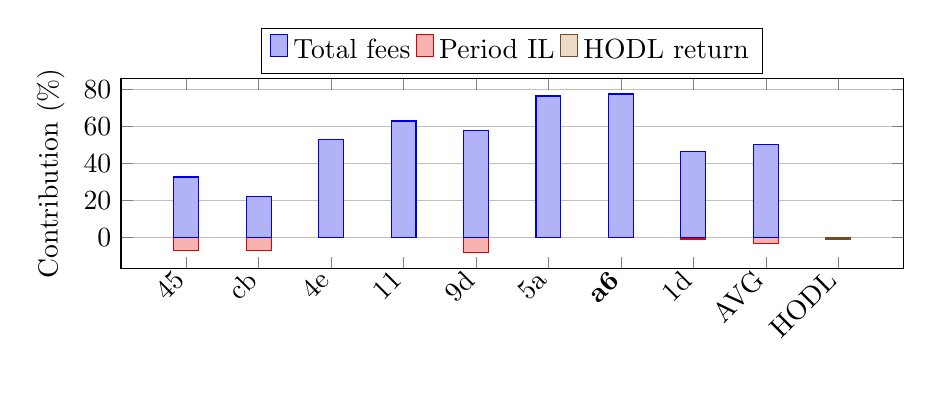
\begin{tikzpicture}
\begin{axis}[
    ybar stacked,
    width=0.95\linewidth,
    height=0.33\textwidth,
    bar width=9pt,
    ylabel={Contribution (\%)},
    symbolic x coords={45,cb,4e,11,9d,5a,a6,1d,AVG,HODL},
    xtick=data,
    xticklabels={45,cb,4e,11,9d,5a,\textbf{a6},1d,AVG,HODL},
    xticklabel style={rotate=45,anchor=east},
    ymajorgrids=true,
    legend style={at={(0.5,1.02)},anchor=south,legend columns=3},
]
\addplot coordinates {
  (45,32.53) (cb,21.93) (4e,52.60) (11,62.77) (9d,57.41) (5a,76.27) (a6,77.39) (1d,46.42)
  (AVG,49.99) (HODL,0.00)
};
\addlegendentry{Total fees}

% 2) Period IL (AVG uses mean across pools; HODL has 0)
\addplot coordinates {
  (45,-7.40) (cb,-7.36) (4e,-0.04) (11,-0.05) (9d,-8.44) (5a,-0.09) (a6,-0.01) (1d,-1.02)
  (AVG,-3.48) (HODL,0.00)
};
\addlegendentry{Period IL}

% 3) HODL return (only HODL is nonzero)
\addplot coordinates {
  (45,0.00) (cb,0.00) (4e,0.00) (11,0.00) (9d,0.00) (5a,0.00) (a6,0.00) (1d,0.00)
  (AVG,0.00) (HODL,-1.00)
};
\addlegendentry{HODL return}
\end{axis}
\end{tikzpicture}
\caption{Pool fees versus IL over 3.5 years (May~2022--Dec~2025). The HODL baseline is shown as a pure price-move contribution (no fees), with a net loss of \(-1\%\) over the same window.}
\label{fig:post_contrib}
\end{figure}



Taken together, \noindent\textit{Tables~\ref{tab:first_year_net90}--\ref{tab:case_bear_bull} and Fig.~\ref{fig:post_contrib} show that the proposed metrics can be used as a practical decision workflow rather than as descriptive statistics}. Using only the first year for calibration, the rules identify a pool that delivers consistently positive \emph{excess} gains across opposite ETH/USD regimes and over a multi-year out-of-sample horizon. 
The decomposition highlights the mechanism---superior outcomes arise when strong fee velocity is paired with controlled divergence risk, whereas high-fee pools can still underperform when structural divergence dominates (as seen in stablecoin-anchored pairs during the drawdown window). Finally, as both fee conditions and correlation regimes evolve over time, this workflow should be applied periodically (e.g., monthly or quarterly) using recent data, rather than committing to a single pool for an entire multi-year horizon.


\section{Conclusion}
\label{sec:conclusion}
In this paper, we study IL in Uniswap v3 to provide LPs with a practical, data-driven way to quantify IL risk and compare pools beyond simple fee-tier heuristics. 
Using multi-year pool data, our IL summaries and predictability diagnostics reveal strong cross-pool differences: Correlated volatile--volatile pairs typically exhibit milder IL, while stable--volatile pools face more systematic divergence-driven losses. These results motivate risk-aware pool selection and horizon management based on both typical outcomes and downside bounds.
In future work, we plan to design and evaluate an adaptive fee model that adjusts fees dynamically in response to changing correlation and historical net performance, aiming to better align LP compensation with time-varying IL risk.

\bibliographystyle{IEEEtran}
\bibliography{references}

\end{document}